\documentclass[a4paper,openright,12pt]{article}
\usepackage[utf8]{inputenc}
\usepackage{graphicx} 
\usepackage{subfigure}
\usepackage[mathscr]{eucal}
\usepackage{titling}
\usepackage{float}
\usepackage{amsmath}
\usepackage{afterpage}
\usepackage{vmargin}
\usepackage[spanish]{babel}
\usepackage{eurosym} 
\usepackage{multirow} 
\usepackage{cite}
\usepackage{url}
\usepackage[colorlinks=true,urlcolor=blue, linkcolor = black, citecolor = blue]{hyperref}


\setlength{\parskip}{1ex} 
\setpapersize{A4}	   %  DIN A4
\setmargins{3cm}    % margen izquierdo
{3.5cm}                     % margen superior
{15cm}                       % anchura del texto
{22.5cm}                   % altura del texto
{10pt}                         % altura de los encabezados
{1cm}                         % espacio entre el texto y los encabezados
{0pt}                           % altura del pie de página
{2cm}                         % espacio entre el texto y el pie de página

\begin{document}

\begin{titlepage}

\begin{center}
\vspace*{-1in}
\begin{figure}[htb]
\begin{center}

\includegraphics[width=8cm]{udc.eps}
\end{center}
\end{figure}

\vspace*{1in}
PROGRAMACIÓN DE SISTEMAS 24/25 Q1\\
Icono de la aplicación\\
\vspace*{1in}
\begin{Large}
\textbf{Juego de air hockey con pantalla dividida} \\
\end{Large}

\vspace*{3in}

\begin{large}
\raggedleft
\textbf{Autores:}\\ José Manuel Fernández Montáns (j.m.fmontans@udc.es) \\
Mateo Rivela Santos (mateo.rivela@udc.es)\\
Hugo Mato Cancela (hugo.matoc@udc.es)\\
\textbf{Persona de contacto:} Hugo\\
\textbf{Fecha:}\textit{ A Coruña, 12 Noviembre 2024}\\
\textbf{Versión:}\textit{1.1}\\
\textbf{Nombre de la aplicación:} \textit{Space Rend Hockey}\\
\textbf{Github:} \url{https://github.com/Hugoomv/TT_PS_Grupo-Q1.1_24-25}\\
\end{large}

\end{center}
\end{titlepage} 

\newpage

\addtocontents{toc}{\hspace{-7.5mm} \textbf{Capítulos}}
\addtocontents{toc}{\hfill \textbf{Página} \par}
\addtocontents{toc}{\vspace{-2mm} \hspace{-7.5mm} \hrule \par}

\pagenumbering{empty}

\tableofcontents

\vspace{5cm}

\begin{flushright}
\begin{table}[hbtp]
\begin{center}

\caption{Tabla de versiones.}
\label{tabla:versiones}
\small
\vspace{1ex}

\begin{tabular}{|c|c|l|}
\hline
Versión & Fecha & Autor \\
\hline \hline
0.1 & 10/10/24 & Hugo\\ \hline
1.0 & 21/10/24 & Hugo\\ \hline
1.1 & 10/11/24 & Hugo\\ \hline
1.2 & 13/11/24 & Hugo\\ \hline
2.0 & 16/11/24 & Hugo\\ \hline

\end{tabular}

\end{center}
\end{table}
\end{flushright}

\newpage
\pagenumbering{arabic}


%%%%%%%
%%%%%%%
\section{Introducción}\label{cap.introduccion}

%%
\subsection{Objetivos}
El objetivo principal será trabajar con una pantalla dividida con una baja latencia y gestionar los rebotes para una pelota que viaja entre dispositivos y añadir un menú.

Podemos añadir notificaciones para que se una alguien a la partida, añadir un ranking, cambiar el tipo de pelota, añadir distintas dificultades iniciales, la pelota que aumente de velocidad con cada rebote de forma indefinida, ver las personas conectadas al juego, poner un estado a cada persona en base a si está en línea o no, o si ya está en una partida.
%%
\subsection{Motivación}
Intención de experimentar con traspaso de datos entre dispositivos e interacción de elementos de la aplicación con la pantalla del dispositivo.
%%
\subsection{Trabajo relacionado}
Existen aplicaciones similares, como es el caso de juegos de air hockey online. Nuestra aplicación busca conectar dos dispositivos de forma remota, a diferencia de las otras aplicaciones, que apuestan por una pantalla dividida para dos jugadores. Destacar que la base del juego es muy parecida, pero sin tener que conectar pantallas.

%%%%%%%
%%%%%%%
\section{Análisis de requisitos}

%%
\subsection{Funcionalidades}
Conectar dos teléfonos, cada uno mostraría una mitad del campo completo, de forma que los elementos en los que cada usuario se tiene que fijar pueden ser de mayor tamaño.
 
Los mazos con los que cada uno tiene que golpear el disco se controlarían con un solo dedo, apareciendo en la parte de la pantalla donde se mantiene este.
 
El disco, al ser golpeado por uno de los mazos, se mueve en una trayectoria determinada por el ángulo (y, preferiblemente, fuerza) del impacto, pudiendo ser alterada al chocar con los límites del campo, que corresponderían a los bordes del dispositivo.
%%
\subsection{Prioridades}
Lo principal sería lograr la conexión entre dispositivos, pasar los datos de forma correcta y apropiada, que el disco pase y rebote para implementar el juego de air hockey.
Primero, se implementará el traspaso de objetos entre pantallas y dispositivos con conexión mediante wifi-internet usando Firebase.
Luego, trabajaremos con rebotes y bordes de la pantalla como paredes.
Una vez realizado lo más básico, añadiremos una pantalla de menú para acceder a los ajustes y a prototipos anteriores. 
Por último, uniremos las funcionalidades básicas, añadiremos bloques destructibles que funcionarán como paredes.

%%%%%%%
%%%%%%%
\section{Planificación inicial}

%%
\subsection{Iteraciones}
Aquí se definen los prototipos de nuestro proyecto y las funcionalidades principales que trabajamos en cada prototipo. Se implementarán en el orden establecido:
\begin{description}
\item[P1:] Pasar un objeto entre dos dispositivos conectados por Wifi-internet usando Firebase.
\item[P2:] Implementar los rebotes y los bordes de la pantalla del dispositivo como paredes en un modo para un jugador.
\item[P3:] Añadimos una maza que el usuario puede manejar y que rebota con la pelota. Sigue siendo en modo para un jugador.
\item[P4:] Añadir un menú con el que acceder a la pantalla de ajustes y a los prototipos anteriores.
\item[P5:] Unión de funcionalidades de P1 y P2: un disco que rebota y se transporta entre dos pantallas al atravesar el borde superior. En ajustes también se podrá cambiar a izquierdo-derecho para tener más tiempo de reacción. 
\item[P6:] Añadir bloques destructibles que funcionen como paredes.
\item[P7:] Producto final
\end{description}
%%
\subsection{Responsabilidades}
\begin{description}

\item[Físicas:] Mateo 
\item[Conexión y Visualización:] José Manuel
\item[Visualización y Entregable:] Hugo
\end{description}

%%
\subsection{Hitos}
\begin{itemize}
\item Crear usuarios en la BD.
\item Login y logout de usuarios.
\item Enviar datos entre dos dispositivos usando Firebase.
\item Establecer una conexión de baja latencia entre ambos dispositivos.
\item Implementar rebotes.
\item Hacer que los bordes de la pantalla funcionen como paredes.
\item Añadir bloques destructibles que funcionen como paredes.
\item Crear un menú con varios ajustes.
\item Crear una partida añadiendo a un jugador mediante invitación.
\item Mostrar un ranking con el número de victorias o puntos.
\item Enseñar el perfil de otros jugadores
\end{itemize}

Entregables:
Cada prototipo será una entrega.

%%
\subsection{Incidencias}
No tenemos conocimientos sobre gráficos o físicas por lo que tendremos que aprender y probar todo lo relacionado a eso. Además, para paliar esas carencias, tenemos pensado usar LibGDX\cite{misc-libGDX} y KryoNet\cite{misc-kryonet} para la codificación general de juego. Y usaremos las librerías Box2d\cite{misc-box2d}, Tween Engine\cite{misc-tween} para las físicas y las animaciones respectivamente. Para establecer conexión se hará uso de Firebase\cite{misc-firebase}. En lo relacionado a Android, tomaremos como referencia lo enseñado en clase y la documentación oficial\cite{misc-android-developers}. Por último, en lo relacionado a los gráficos y apartado más visual, Canva \cite{misc-canva}.
\par
En la primera iteración, probaremos la conexión entre dispositivos y que el objeto se pasa correctamente entre ellos.
En la segunda, en un prototipo distinto, el objeto debe rebotar contra los bordes de la pantalla de un dispositivo para que funcionen como paredes
En la tercera, implementamos la maza, que debe responder correctamente al input del usuario, y nos aseguramos que la pelota rebote correctamente contra esta.
En la cuarta, el menú nos debe permitir cambiar entre varios prototipos
En la quinta, uniremos las funcionalidades de las dos primeras iteraciones y nos aseguraremos de que funcionan correctamente ambas al mismo tiempo
En la sexta, añadiremos bloques que funcionen como paredes. La pelota debe rebotar contra estos como lo hace con los bordes de la pantalla.
En la última, comprobaremos que, tras haber implementado todo, funciona correctamente.
\par
En caso de que alguien enferme repartiremos el trabajo asignado a esa persona entre los demás integrantes del grupo.

%%%%%%%
%%%%%%%
\section{Diseño}
\subsection{Arquitectura}
Se hará uso de una arquitectura centralizada cliente servidor. La distribución de trabajo se hará entre el servidor (Firebase) y el cliente (el usuario de nuestra app). El servidor almacena la información de los usuarios, y los mensajes que envían. Guardará datos como si el usuario está conectado o no, su id (único para cada uno), nombre, correo y contraseña. El cliente revisa el usuario actual, con el que estamos logueados, en el servidor y tiene un listener que escucha los cambios, como son los mensajes recibidos por otros usuarios.


\subsection{Persistencia}
Respecto a qué información almacenaremos, ambos jugadores siempre tendrán los datos de la posición, ángulo y fuerza de la pelota. Además, cada uno guardará dónde está situada su propia maza en caso de que esté siendo usada. El servidor guardará las coordenadas de la pelota, que los usuarios obtendrán de forma constante. \\
Mientras el usuario está conectado, podrá recibir datos, invitaciones o mensajes y se mostrará como online. Una vez que esté fuera de línea, no será posible que reciba nada de lo anterior. Cuando vuelva a conectarse, se actualizará y cargará los mensajes que recibió mientras estaba offline.

\subsection{Vista}
En lo que respecta al diseño de la aplicación, tendremos una única actividad a priori en la que, mediante fragmentos, iremos añadiendo la dinámica. El manejo del juego en sí se hará mediante un view personalizado, mostrando todos los elementos y actualizando sus respectivas posiciones cada cierto tiempo. \\
En la primera pantalla el usuario se podrá loguear o registrar. Introducirá su email y su contraseña. Una vez dentro, en la pantalla principal se mostrarán varios botones: 
\begin{itemize}
    \item Jugar: Permitirá iniciar el juego en modo solitario o en línea.
    \item Ajustes: Mostrará un menú con varias opciones que modificar, como cambiar la orientación de la pantalla.
    \item Invitar: Abrirá un desplegable para poder iniciar una partida con otro usuario.
\end{itemize}

\begin{figure}[htp]
    \centering
    \begin{minipage}{0.45\textwidth}
        \centering
        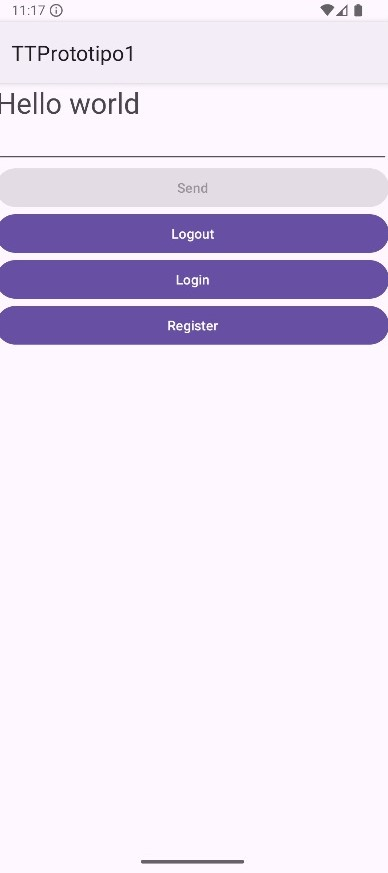
\includegraphics[width=\textwidth]{Images/Vista_It1.jpg}
        \caption{Figura 1}
        \label{fig:Pantalla de inicio}
    \end{minipage}
    \hfill
    \begin{minipage}{0.45\textwidth}
        \centering
        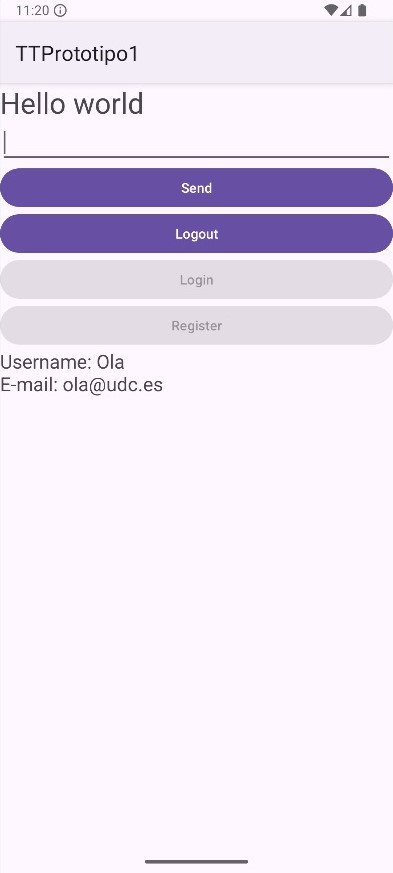
\includegraphics[width=\textwidth]{Images/Vista_It1_2.jpg}
        \caption{Pantalla una vez logueado}
        \label{fig:figura2}
    \end{minipage}
    \caption{Pantallas de la primera iteración}
    \label{fig:side_by_side}
\end{figure}


\subsection{Comunicaciones}
La comunicación en este juego es una parte fundamental. Para ello, buscamos un sistema de baja latencia. Para esta conexión, se contará con un servidor central al que cada cliente se conectará por internet (Firebase), de esta forma, se gana en rango de uso (rango global). Existe un claro problema y es que el servidor del que se va a hacer uso es gratuito y, por lo tanto, la latencia va a ser bastante alta, pero hemos llegado a la conclusión de que es no es crítico para este proyecto porque, como cada usuario en una partida solo va a ver su pantalla a priori. En el caso de que ambos jugadores estén juntos físicamente, la latencia sería notable.

\subsection{Sensores}
Se hace uso de la pantalla táctil, con este se implementará el movimiento del mazo en cuestión. Es un dispositivo que detecta y responde al contacto físico o la presión sobre su superficie, en este caso no se hará uso de la detección de la presión. Para la implementación del rebote se puede tener o no en cuenta la velocidad con la que se desplaza en contacto con el panel táctil pero no es algo que vayamos a implementar en nuestro caso desde a priori.
\subsection{Trabajo en background}
Se enviarán los datos de la posición y ángulo de la pelota, cada X tiempo. Se usa Firebase para trabajar con una comunicación y latencia en tiempo real. Para controlar la velocidad de actualización de la pantalla y evitar sobrecargar la CPU, usaremos un servicio que recibirá las coordenadas del servidor. Con cada nueva información, se modificará la posición de la pelota en la pantalla.

\section{Arquitectura Propuesta}
Ahora mismo es una aplicación monolítica y cambiará a CLEAN Arquitecture. En esta primera iteración hay una actividad principal que incluye todo, user y UsersAdapter para el ListView que muestra los usuarios conectados. 

\section{Diseño e implementación de la 1ª iteración}
Se ha creado una aplicación con una MainActivity, UsersAdapters y User. Partimos de un diseño monolítico, que en un futuro pasará a ser CLEAN Arquitecture. En la MainActivity está la mayor parte del código, como es la UI. La interfaz incluye en la parte superior un TextView que mostrará los mensajes que recibamos de otros jugadores. Después, un EditText donde escribir el mensaje que queremos enviar a otros jugadores. Más abajo, están cuatro botones. Por último, un TextView con nuestro nombre de usuario y el email. Este último TextView no mostrará nada si el usuario no está logueado. Además, se ha añadido toast para informar al usuario si hay problemas al iniciar sesión, conectarse...
A continuación se explica el funcionamiento de los botones:
\begin{itemize}
    \item Send: muestra un desplegable con los usuarios conectados a los que podemos enviar un mensaje. Deshabilitado si el usuario no ha iniciado sesión.
    \item Logout: permite cerrar sesión.
    \item Login: iniciar sesión. Muestra AlertDialog para introducir los datos, correo y contraseña. Además, aparece un botón para cambiar a register. Deshabilitado si el usuario ya ha iniciado sesión.
    \item Register: registrar usuario. Muestra un AlertDialog similar al de login y también tiene el botón para alternar a login. Deshabilitado si el usuario ya ha iniciado sesión.
\end{itemize}

UsersAdapters y Users es usado para la implementación del ListView que muestra los usuarios conectados (tras pulsar Send). La app se conecta a Firebase, donde se han creado varios usuarios para comprobar que funciona correctamente, con su login y logout, y se ha implementado el envío de mensajes, lo que representaría a los primeros hitos.
Finalmente, también se ha inicializado la base de datos haciendo uso del json.

\section{$1^{ras} \text{ pruebas}$}
Se han usado dos emuladores en la misma máquina para comprobar el funcionamiento de la aplicación. Se han comprobado el registro de usuarios, el login, el logout, la creación de datos en la base de datos en tiempo real y el paso de mensajes usando Firebase. Adicionalmente, se han usado varios equipos distintos, y se han comunicado varias apps de emuladores y equipos diferentes.

%%%%%%%

\section{Bibliografía}
\bibliographystyle{pfc-fic}
\bibliography{biblio}


\end{document}